\documentclass[12pt,a4paper]{article}

\usepackage[utf8]{inputenc}
\usepackage[T1]{fontenc}
\usepackage[brazil]{babel}
\usepackage{geometry}
\usepackage{graphicx}
\usepackage{float}
\usepackage{xcolor}
\usepackage{hyperref}
\usepackage{booktabs}
\usepackage{longtable}
\usepackage{array}
\usepackage{listings}
\usepackage{tikz}
\usepackage{fancyhdr}
\usepackage{caption}

\usetikzlibrary{arrows.meta, positioning, shapes.geometric, fit, calc}

\geometry{left=3cm,right=2cm,top=3cm,bottom=2cm}    
\setlength{\emergencystretch}{3em}

\hypersetup{
    colorlinks=true,
    linkcolor=blue!55!black,
    urlcolor=blue!65!black,
    citecolor=blue!55!black,
    pdftitle={Sistema de Inspecao Automatica de Tuneis - Relatorio Final},
    pdfauthor={Leandro Lopo e Rodrigo Martins}
}

\pagestyle{fancy}
\fancyhf{}
\fancyhead[L]{Sistema de Inspeção Automática de Túneis}
\fancyhead[R]{Automação em Tempo Real}
\fancyfoot[C]{\thepage}
\setlength{\headheight}{15pt}

\definecolor{codegray}{RGB}{247,247,247}
\definecolor{codeborder}{RGB}{205,205,205}
\definecolor{codecomment}{RGB}{60,115,70}
\definecolor{codekeyword}{RGB}{0,75,145}
\definecolor{codestring}{RGB}{155,55,35}
\definecolor{archblue}{RGB}{222,235,250}
\definecolor{archgreen}{RGB}{220,242,224}
\definecolor{archyellow}{RGB}{255,243,199}
\definecolor{archred}{RGB}{250,220,220}

\lstdefinestyle{basecode}{
    basicstyle=\ttfamily\scriptsize,
    keywordstyle=\color{codekeyword}\bfseries,
    commentstyle=\color{codecomment},
    stringstyle=\color{codestring},
    backgroundcolor=\color{codegray},
    frame=single,
    rulecolor=\color{codeborder},
    numbers=left,
    numberstyle=\tiny\color{gray},
    numbersep=7pt,
    breaklines=true,
    breakatwhitespace=false,
    columns=fullflexible,
    keepspaces=true,
    tabsize=4,
    showstringspaces=false,
    captionpos=b,
    inputencoding=utf8,
    literate=
        {á}{{\'a}}1 {à}{{\`a}}1 {ã}{{\~a}}1 {â}{{\^a}}1
        {Á}{{\'A}}1 {À}{{\`A}}1 {Ã}{{\~A}}1 {Â}{{\^A}}1
        {é}{{\'e}}1 {ê}{{\^e}}1 {É}{{\'E}}1 {Ê}{{\^E}}1
        {í}{{\'i}}1 {Í}{{\'I}}1
        {ó}{{\'o}}1 {õ}{{\~o}}1 {ô}{{\^o}}1
        {Ó}{{\'O}}1 {Õ}{{\~O}}1 {Ô}{{\^O}}1
        {ú}{{\'u}}1 {Ú}{{\'U}}1
        {ç}{{\c{c}}}1 {Ç}{{\c{C}}}1
        {²}{{$^2$}}1
}

\lstdefinestyle{cppstyle}{style=basecode,language=C++}
\lstdefinestyle{pythonstyle}{style=basecode,language=Python}
\lstdefinestyle{textstyle}{
    style=basecode,
    numbers=none,
    keywordstyle=,
    commentstyle=,
    stringstyle=
}

\newcommand{\codigo}[2]{
    \subsection{\texttt{#1}}
    \lstinputlisting[style=cppstyle]{#2}
}

\newcommand{\codigopython}[2]{
    \subsection{\texttt{#1}}
    \lstinputlisting[style=pythonstyle]{#2}
}

\begin{document}

\pagenumbering{gobble}
\begin{titlepage}
    \centering
    \vspace*{1.5cm}
    {\Large Universidade Federal de Minas Gerais\par}
    \vspace{0.4cm}
    {\large Automação em Tempo Real\par}
    \vspace{2.0cm}
    {\Huge\bfseries Sistema de Inspeção Automática de Túneis\par}
    \vspace{0.6cm}
    {\Large Relatório Final\par}
    \vspace{2.3cm}

    \begin{tabular}{ll}
        \textbf{Leandro Lopo} & Matrícula 2021020520 \\
        \textbf{Rodrigo Martins} & Matrícula 2023421459
    \end{tabular}

    \vfill
    Professor: Leandro Freitas\par
    \vspace{0.5cm}
    Belo Horizonte\par
    2026
\end{titlepage}

\pagenumbering{roman}
\tableofcontents
\clearpage
\listoffigures
\clearpage
\pagenumbering{arabic}

\section{Introdução}

O projeto implementa um sistema simulado de inspeção automática do teto de um túnel. Um robô móvel recebe comandos de aceleração, mede sua velocidade, detecta transições de encoder e lê a distância até o teto por LIDAR. O núcleo combina posição e distância para reconstruir o perfil do túnel. Uma variação superior ao limite configurado caracteriza uma possível falha, reduz a velocidade e aciona uma tarefa de inspeção por câmera.

A solução é formada por três programas: núcleo concorrente em C++, simulação gráfica em Python/Pygame e operação remota em Python/Pygame. O broker Mosquitto realiza a comunicação entre processos por MQTT. Internamente, o núcleo usa threads, filas produtor--consumidor, mutexes, variáveis de condição e tarefas periódicas, aplicando diretamente os conteúdos de programação concorrente, sincronização, entrada e saída assíncrona, IPC e sistemas de tempo real estudados na disciplina.

\begin{figure}[H]
    \centering
    \begin{tikzpicture}[
        x=0.88cm,
        y=0.88cm,
        robot/.style={draw,thick,fill=gray!20,minimum width=1.7cm,minimum height=0.7cm},
        sensor/.style={-{Latex[length=3mm]},thick,green!50!black}
    ]
        \fill[gray!9] (0,0) rectangle (13,5.2);
        \draw[very thick] (0,0.3) -- (13,0.3);
        \draw[very thick,blue!65!black]
            (0,4.4) -- (3.4,4.4)
            .. controls (3.7,3.4) and (4.6,3.4) .. (4.9,4.4)
            -- (8.1,4.4)
            .. controls (8.4,5.0) and (9.3,5.0) .. (9.6,4.4)
            -- (13,4.4);
        \node[robot] (robo) at (6.4,0.75) {robô};
        \draw[sensor] (6.4,1.1) -- (6.4,4.4) node[midway,right] {LIDAR};
        \draw[red!70!black,very thick] (3.4,4.4)
            .. controls (3.7,3.4) and (4.6,3.4) .. (4.9,4.4);
        \node[red!70!black,align=center] at (4.15,2.7) {cavidade\\severa};
        \node[align=center] at (9.0,3.7) {saliência\\menor};
        \draw[-{Latex[length=3mm]},thick] (1,0.0) -- (12,0.0) node[right] {$x$};
    \end{tikzpicture}
    \caption{Ilustração própria do problema: inspeção do perfil do teto por um robô com LIDAR.}
    \label{fig:problema}
\end{figure}

\subsection{Objetivos}

Os objetivos principais são:

\begin{itemize}
    \item simular o movimento do robô, o encoder, o LIDAR e irregularidades do teto;
    \item executar controle automático PID e permitir comandos manuais remotos;
    \item reconstruir e registrar o perfil do túnel durante o percurso;
    \item detectar variações severas, acionar a câmera e reduzir a velocidade;
    \item distribuir tarefas concorrentes com acesso seguro aos dados compartilhados;
    \item integrar C++ e Python por comunicação MQTT assíncrona;
    \item avaliar funcionamento, capacidade e limitações temporais do protótipo.
\end{itemize}

\section{Proposta de Arquitetura}

\subsection{Visão geral}

A arquitetura final separa interface física simulada, processamento e supervisão. Essa separação evita acoplar a taxa de desenho das interfaces ao núcleo de controle e permite iniciar cada processo de maneira independente.

\begin{figure}[H]
    \centering
    \begin{tikzpicture}[
        node distance=1.1cm and 1.4cm,
        bloco/.style={draw,rounded corners=2pt,minimum width=3.4cm,minimum height=1.25cm,align=center,thick},
        fluxo/.style={-{Latex[length=2.6mm]},thick},
        mqtt/.style={draw,diamond,aspect=2.1,fill=archyellow,align=center,thick}
    ]
        \node[bloco,fill=archgreen] (sim) {Simulação\\Python + Pygame};
        \node[mqtt,right=of sim] (broker) {Broker MQTT\\localhost:1883};
        \node[bloco,fill=archblue,right=of broker] (core) {Núcleo concorrente\\C++ + 11 threads};
        \node[bloco,fill=archgreen,below=of broker] (remote) {Operação remota\\Python + Pygame};
        \node[bloco,fill=gray!15,below=of core] (csv) {Registro local\\\texttt{surface\_points.csv}};

        \draw[fluxo] (sim) -- node[above,align=center]{sensores\\JSON} (broker);
        \draw[fluxo] (broker) -- node[above,align=center]{sensores e\\comandos} (core);
        \draw[fluxo] (core) to[bend left=14] node[below]{atuadores} (broker);
        \draw[fluxo] (broker) to[bend left=14] (sim);
        \draw[fluxo] (remote) -- node[left]{comandos} (broker);
        \draw[fluxo] (broker) to[bend right=15] node[right]{estado e superfície} (remote);
        \draw[fluxo] (core) -- (csv);
    \end{tikzpicture}
    \caption{Arquitetura final distribuída em processos e comunicação MQTT.}
    \label{fig:arquitetura-final}
\end{figure}

\begin{longtable}{p{3.2cm}p{4.2cm}p{6.5cm}}
\caption{Processos e responsabilidades da arquitetura.}
\label{tab:processos}\\
\toprule
\textbf{Processo} & \textbf{Tecnologia} & \textbf{Responsabilidade} \\
\midrule
\endfirsthead
\toprule
\textbf{Processo} & \textbf{Tecnologia} & \textbf{Responsabilidade} \\
\midrule
\endhead
Simulação & Python, Pygame e Paho MQTT & Integra dinâmica do robô a cada 80 ms, gera encoder/LIDAR com ruído, publica sensores e aplica os atuadores recebidos. \\
Núcleo & C++17, \texttt{std::thread}, libmosquitto e nlohmann/json & Executa controle, cálculo de posição, reconstrução, detecção, câmera, coleta e gateways MQTT. \\
Operação remota & Python, Pygame e Paho MQTT & Envia modo, direção, setpoint e limite de falha, além de exibir o estado e a superfície reconstruída. \\
Broker & Mosquitto & Desacopla publishers e subscribers usando tópicos MQTT. \\
\bottomrule
\end{longtable}

A Tabela~\ref{tab:processos} evidencia a separação entre planta simulada, decisão de controle e supervisão. A \textbf{simulação} representa a parte física: integra aceleração e velocidade, movimenta o robô e produz os sinais que, em uma aplicação real, viriam dos sensores. Ela também recebe os comandos calculados pelo núcleo, fechando a malha de controle. O período de 80 ms foi mantido igual ao do controlador para que cada atualização física possa gerar uma nova amostra coerente.

O \textbf{núcleo C++} concentra as funções que exigem ordem, sincronização e resposta previsível. Como ele não desenha interfaces, dedica-se a receber dados, executar o controle, reconstruir a superfície e produzir atuadores. Essa separação impede que variações na taxa de quadros do Pygame atrasem diretamente o PID. A \textbf{operação remota} atua como supervisório, alterando parâmetros e apresentando resultados sem participar do cálculo de cada ciclo. Assim, o robô continua processando as últimas configurações válidas mesmo que a janela remota demore para redesenhar.

O \textbf{broker Mosquitto} elimina conexões diretas entre cada par de programas. Cada processo conhece apenas os tópicos que publica ou assina, o que facilita substituir a simulação por sensores reais ou executar a operação remota em outra máquina. O CSV complementa essa arquitetura com uma saída persistente e independente da interface gráfica. Dessa maneira, os pontos já coletados permanecem disponíveis para análise mesmo depois que a janela é fechada.

\subsection{Comunicação MQTT}

O MQTT foi adotado como IPC porque os três programas são processos independentes e usam linguagens diferentes. O broker é executado em \texttt{localhost:1883}. O núcleo C++ se conecta por libmosquitto, enquanto as interfaces Python usam Paho MQTT. As mensagens são codificadas em JSON, formato diretamente suportado nas duas linguagens e legível durante a depuração. O protótipo usa QoS 0, suficiente para a execução local, mas sem confirmação de entrega.

\begingroup
\small
\begin{longtable}{p{4.2cm}p{3.3cm}p{2.4cm}p{3.4cm}}
\caption{Tópicos MQTT implementados.}
\label{tab:mqtt}\\
\toprule
\textbf{Tópico} & \textbf{Origem $\rightarrow$ destino} & \textbf{Período} & \textbf{Campos principais} \\
\midrule
\endfirsthead
\toprule
\textbf{Tópico} & \textbf{Origem $\rightarrow$ destino} & \textbf{Período} & \textbf{Campos principais} \\
\midrule
\endhead
\texttt{atr/sim/sensors} & Simulação $\rightarrow$ núcleo & 80 ms & encoder, LIDAR, velocidade, posição real e timestamp \\
\texttt{atr/core/actuators} & Núcleo $\rightarrow$ simulação & 80 ms & aceleração e câmera \\
\texttt{atr/remote/commands} & Operação $\rightarrow$ núcleo & por comando & modo, direção, parada, setpoint e limite \\
\texttt{atr/core/state} & Núcleo $\rightarrow$ operação & 80 ms & modo, inspeção, posição, velocidade e atuadores \\
\texttt{atr/core/surface} & Núcleo $\rightarrow$ operação & por amostra & timestamp, posição, LIDAR filtrado e confiança \\
\bottomrule
\end{longtable}
\endgroup

Os cinco tópicos da Tabela~\ref{tab:mqtt} formam dois fluxos principais. O primeiro corresponde à \textbf{malha robô--núcleo}. A cada ciclo, \texttt{atr/sim/sensors} entrega encoder, LIDAR e velocidade ao núcleo. Depois do processamento, \texttt{atr/core/actuators} devolve aceleração e estado da câmera. Como ambos são publicados a cada 80 ms, a simulação recebe comandos na mesma escala de tempo usada pelo controlador.

O segundo fluxo é de \textbf{supervisão}. \texttt{atr/remote/commands} só é publicado quando o operador altera modo, direção, parada, setpoint ou limite de falha, evitando tráfego periódico sem mudança. No sentido contrário, \texttt{atr/core/state} envia uma visão consolidada do robô a cada 80 ms, suficiente para atualizar os indicadores da interface. Já \texttt{atr/core/surface} é orientado a dados: cada ponto reconstruído é publicado assim que fica pronto, permitindo que o gráfico cresça durante o percurso.

Os campos de cada mensagem acompanham a função do tópico. O \texttt{timestamp} preserva a referência temporal, enquanto encoder e LIDAR alimentam a reconstrução. A velocidade fecha a realimentação do PID, e os campos de posição, confiança e inspeção atualizam a interface. As publicações usam QoS 0 e não são retidas. Essa escolha reduz a sobrecarga porque uma amostra antiga pode ser substituída pela seguinte, mas não oferece garantia de entrega. Em uma aplicação crítica, seria necessário usar QoS 1, números de sequência e uma estratégia de reconexão.

O receptor valida e converte o JSON dentro de \texttt{try--catch}. Uma mensagem malformada é registrada e descartada sem terminar o processo. O campo \texttt{finalizado} encerra o pipeline e acorda consumidores ainda bloqueados.

\begin{lstlisting}[style=cppstyle,caption={Conversão do payload MQTT em dados internos.}]
try {
    const json mensagem = json::parse(payload);
    SensorData leitura;
    leitura.i_encoder = mensagem.at("i_encoder").get<bool>();
    leitura.i_lidar = mensagem.at("i_lidar").get<int>();
    leitura.timestamp = mensagem.at("timestamp").get<double>();
    // O mesmo evento alimenta os fluxos de LIDAR e encoder.
}
catch (const std::exception &erro) {
    std::cerr << "Erro ao interpretar mensagem MQTT: "
              << erro.what() << std::endl;
}
\end{lstlisting}

\subsection{Threads do núcleo}

O arquivo \texttt{src/main.cpp} cria os buffers, estados e 11 threads, passa referências com \texttt{std::ref} e usa \texttt{join()} para controlar o encerramento. As tarefas estão agrupadas abaixo.

\begingroup
\small
\begin{longtable}{p{5.4cm}p{2.1cm}p{5.8cm}}
\caption{Tarefas concorrentes do núcleo.}
\label{tab:threads}\\
\toprule
\textbf{Tarefa} & \textbf{Ativação} & \textbf{Função} \\
\midrule
\endfirsthead
\toprule
\textbf{Tarefa} & \textbf{Ativação} & \textbf{Função} \\
\midrule
\endhead
\texttt{ComandoNavegacao} & 80 ms & Atualiza o modo automático/manual do estado global. \\
\texttt{ControleNavegacao} & 80 ms & Executa PID ou comando manual e gera aceleração. \\
\texttt{RecebeSensoresMqtt} & evento MQTT & Converte sensores e produz duas filas internas. \\
\texttt{RecebeComandosMqtt} & evento MQTT & Atualiza comando e limite de falha. \\
\texttt{PublicaAtuadoresMqtt} & 80 ms & Envia aceleração e câmera à simulação. \\
\texttt{PublicaEstadoMqtt} & 80 ms & Envia telemetria à operação remota. \\
\texttt{DistanciaPercorrida} & evento & Converte transições do encoder em posição. \\
\texttt{ReconstrucaoSuperficie} & evento & Filtra LIDAR, combina posição e detecta falha. \\
\texttt{ColetorDados} & evento & Calcula confiança e grava CSV. \\
\texttt{PublicaSuperficieMqtt} & evento & Envia cada ponto à interface remota. \\
\texttt{InspecaoCamera} & evento de falha & Executa carga computacional por aproximadamente 2 s. \\
\bottomrule
\end{longtable}
\endgroup

As tarefas da Tabela~\ref{tab:threads} foram divididas em três grupos. O primeiro contém as tarefas \textbf{periódicas}: \texttt{ComandoNavegacao}, \texttt{ControleNavegacao}, \texttt{PublicaAtuadoresMqtt} e \texttt{PublicaEstadoMqtt}. Todas usam período de 80 ms. O comando consolida o modo solicitado, o controle calcula a aceleração e os dois publishers enviam, respectivamente, a saída para a planta e a telemetria para o supervisório. Essa separação mantém o cálculo do PID independente do tempo gasto na comunicação.

O segundo grupo é \textbf{orientado à chegada de dados}. \texttt{RecebeSensoresMqtt} transforma um payload em duas entradas, uma para o encoder e outra para o LIDAR. Em seguida, \texttt{DistanciaPercorrida} converte as transições do encoder em posição, que é combinada com a leitura de distância por \texttt{ReconstrucaoSuperficie}. O ponto resultante é enviado tanto a \texttt{ColetorDados} quanto a \texttt{PublicaSuperficieMqtt}. Em paralelo, \texttt{RecebeComandosMqtt} altera os estados usados pelas próximas execuções periódicas. Enquanto não há trabalho, essas threads permanecem bloqueadas em vez de consultar filas continuamente.

O terceiro grupo trata a \textbf{inspeção excepcional}. Ao detectar uma variação acima do limite, a reconstrução sinaliza \texttt{InspecaoCamera}. O processamento de aproximadamente 2 s ocorre em uma thread própria porque é muito maior que o período de controle. Dessa forma, a câmera consome CPU sem manter mutexes do pipeline e sem bloquear diretamente a produção dos próximos comandos de aceleração.

Com essa divisão, os dados seguem do sensor MQTT para os buffers de sensor e encoder. Depois passam pelo cálculo de posição e pela reconstrução, que produz o CSV, a superfície remota e, quando necessário, o evento de câmera. Na finalização, as flags dos buffers e as notificações acordam as tarefas bloqueadas. O \texttt{main} então espera cada thread com \texttt{join()} antes de liberar a biblioteca MQTT, evitando que algum consumidor permaneça aguardando um produtor já encerrado.

\subsection{Sincronização}

O núcleo compartilha filas, comandos, parâmetros, estados e atuadores entre threads. Sem sincronização, duas operações poderiam modificar a mesma estrutura ao mesmo tempo, uma tarefa poderia ler um estado parcialmente atualizado ou um consumidor poderia tentar retirar um item enquanto o produtor altera a fila. A estratégia adotada foi separar os dados por função e associar um mutex próprio a cada estrutura, reduzindo o número de threads que competem pela mesma seção crítica.

Os estados de robô, comando, atuadores, parâmetros e controle do sistema usam \texttt{std::lock\_guard}. A thread trava o mutex, copia o conjunto de campos para variáveis locais e libera a proteção antes de realizar cálculos ou comunicação. Esse padrão produz uma fotografia coerente do estado e mantém operações mais lentas, como JSON, MQTT, escrita em arquivo e processamento da câmera, fora da região crítica.

Para dados sequenciais, as filas seguem o padrão produtor--consumidor. Cada uma contém \texttt{std::queue}, \texttt{std::mutex}, \texttt{std::condition\_variable} e flag de finalização. A fila preserva a ordem das amostras e desacopla pequenas diferenças de velocidade entre produtor e consumidor. O mutex protege apenas a inserção ou retirada. Depois que ele é liberado, a thread executa filtragem, cálculo e I/O sem aumentar a contenção.

\begin{lstlisting}[style=cppstyle,caption={Estrutura de fila sincronizada.}]
struct SensorBuffer {
    std::queue<SensorData> fila_sensor;
    std::mutex mutex_sensor;
    std::condition_variable dado_disponivel_var;
    bool finalizado = false;
};
\end{lstlisting}

O consumidor usa \texttt{std::unique\_lock}, necessário porque \texttt{wait()} libera o mutex ao bloquear e o readquire ao acordar. Enquanto a fila está vazia, a thread não consome CPU. O predicado trata tanto dado disponível quanto finalização e também protege contra despertares espúrios: acordar não significa automaticamente que há uma amostra válida.

\begin{lstlisting}[style=cppstyle,caption={Espera bloqueante sem polling.}]
std::unique_lock<std::mutex> trava(buffer.mutex_sensor);
buffer.dado_disponivel_var.wait(trava, [&buffer] {
    return !buffer.fila_sensor.empty() || buffer.finalizado;
});

if (buffer.fila_sensor.empty() && buffer.finalizado) {
    break;
}

leitura = buffer.fila_sensor.front();
buffer.fila_sensor.pop();
\end{lstlisting}

\texttt{std::lock\_guard} aplica RAII às seções críticas simples, fazendo com que o desbloqueio ocorra automaticamente ao sair do escopo, inclusive em exceções. Isso reduz erros de desbloqueio, mas não elimina por si só a possibilidade de deadlock. Por esse motivo, o código evita manter dois mutexes simultaneamente. Quando uma tarefa precisa ler comando e estado, cada estrutura é copiada em um escopo separado, sem criar dependência circular entre travas.

\texttt{notify\_one()} acorda um único consumidor quando chega uma amostra, pois cada fila normal possui um destino definido. Já \texttt{notify\_all()} é reservado à finalização, quando todas as threads bloqueadas precisam reavaliar seus predicados. Antes da notificação, a flag \texttt{finalizado} é alterada sob o mesmo mutex da fila. Essa ordem evita a perda do sinal de término entre a verificação do predicado e o bloqueio. O evento da câmera usa a mesma estratégia, enquanto o callback MQTT utiliza \texttt{std::atomic<bool>} para a flag consultada fora dos mutexes dos buffers.

Dois \texttt{SurfaceBuffer} independentes realizam o \textit{fan-out} da reconstrução. Um alimenta o CSV e o outro alimenta o publisher MQTT. Se houvesse apenas uma fila com dois consumidores, os pontos seriam divididos entre eles em vez de enviados aos dois destinos. De forma semelhante, o callback de sensores produz \texttt{SensorData} e \texttt{EncoderData} em filas separadas. Assim, reconstrução e distância avançam de forma independente, sem perder a ordem correspondente das amostras.

Na prática, cada mecanismo cobre uma necessidade específica. O mutex fornece exclusão mútua, a variável de condição sinaliza trabalho sem polling e a flag ou valor atômico torna o encerramento observável. Não foram usados semáforos porque a própria fila armazena a quantidade e o conteúdo do trabalho pendente. Nesse caso, o predicado da variável de condição expressa diretamente quando o consumidor pode prosseguir.

\subsection{Periodicidade}

O sistema combina tarefas periódicas e tarefas esporádicas. Controle, interpretação de comando, publicação de atuadores e publicação de estado executam a cada 80 ms, equivalentes a 12,5 Hz. Para essas tarefas foi assumido prazo igual ao período: o cálculo e a publicação de um ciclo devem terminar antes da próxima ativação. A física simulada usa o mesmo intervalo, mantendo alinhadas a geração de sensores e a atualização do controle. A interface gráfica pode redesenhar a 60 quadros/s, mas isso não altera o passo físico de 80 ms.

As demais tarefas não precisam acordar periodicamente. Recepção MQTT, distância, reconstrução, coleta, publicação da superfície e câmera são ativadas pela chegada de mensagem, disponibilidade na fila ou evento de falha. Essa divisão evita reservar ciclos para tarefas sem dados e reduz uso de CPU quando o sistema está ocioso.

As tarefas cíclicas usam \texttt{std::chrono::steady\_clock} e \texttt{sleep\_until}. O relógio monotônico não sofre saltos por ajustes do relógio civil. O instante seguinte é incrementado a partir da referência anterior, evitando acumular diretamente o tempo de processamento de cada ciclo, como ocorreria com chamadas sucessivas de \texttt{sleep\_for}.

\begin{lstlisting}[style=cppstyle,caption={Padrão usado nas tarefas periódicas.}]
auto proximaExecucao = std::chrono::steady_clock::now();
while (sistemaRodando) {
    proximaExecucao += std::chrono::milliseconds(80);
    // Leitura, calculo e publicacao.
    std::this_thread::sleep_until(proximaExecucao);
}
\end{lstlisting}

Em cada iteração, a tarefa calcula primeiro o próximo instante, executa seu trabalho e dorme apenas pelo tempo restante. Se o processamento ultrapassar 80 ms, \texttt{sleep\_until} retorna imediatamente porque o prazo já passou. Nesse caso, o código inicia o próximo ciclo sem espera para tentar recuperar a referência periódica. Como o protótipo não descarta ciclos nem registra automaticamente cada estouro, a análise temporal posterior mede os custos e verifica a margem disponível em relação ao período.

A câmera é o caso de maior duração, com cerca de 2 s de processamento. Como esse tempo violaria o prazo de uma tarefa periódica, a inspeção foi implementada em uma thread orientada a evento. O escalonador pode então executá-la em paralelo com o controle. Ainda assim, \texttt{std::thread} sobre Linux com política normal não oferece garantia de tempo real rígido. O período de 80 ms é uma configuração validada experimentalmente, e não um WCET formal. Essa distinção é retomada na análise de capacidade e escalabilidade.

\section{Implementação}

\subsection{Controle de navegação}

No modo automático, \texttt{ControleNavegacao} calcula erro, integral limitada e derivada a cada 80 ms. A saturação reduz o \textit{windup}, enquanto a limitação da saída mantém a aceleração no intervalo $[-100,100]$. Durante a inspeção, o setpoint máximo passa a 1 m/s. No modo manual, os comandos direita, esquerda e parada geram diretamente aceleração positiva, negativa ou nula.

\begin{lstlisting}[style=cppstyle,caption={Núcleo do controlador PID.}]
const double erro = setpointVelocidade - velocidadeAtual;
integralErro = std::clamp(
    integralErro + erro * periodoSegundos,
    -limiteIntegral,
    limiteIntegral
);
const double derivadaErro = (erro - erroAnterior) / periodoSegundos;
const double saidaPid = kp * erro + ki * integralErro + kd * derivadaErro;
const int aceleracao = static_cast<int>(
    std::clamp(saidaPid, -100.0, 100.0)
);
\end{lstlisting}

\subsection{Posição e reconstrução}

\texttt{DistanciaPercorrida} detecta mudanças no nível lógico do encoder. Cada transição representa um metro. O sinal da velocidade define avanço ou retorno, e a posição é limitada a zero. Para cada leitura é produzido um \texttt{PositionData}, inclusive quando não ocorre transição, mantendo correspondência um-para-um com as leituras do LIDAR.

\texttt{ReconstrucaoSuperficie} retira uma amostra de sensor e uma amostra de posição, aplica média móvel de janela 3 ao LIDAR e cria um ponto $(x,y)$. A média reduz ruído sem exigir armazenamento completo do percurso.

\begin{lstlisting}[style=cppstyle,caption={Média móvel de três leituras.}]
ultimasLeituras.push(leitura.i_lidar);
somaLeituras += leitura.i_lidar;

if (ultimasLeituras.size() > tamanhoJanela) {
    somaLeituras -= ultimasLeituras.front();
    ultimasLeituras.pop();
}

const double mediaMovel =
    static_cast<double>(somaLeituras) / ultimasLeituras.size();
\end{lstlisting}

\subsection{Detecção e câmera}

A detecção compara leituras brutas consecutivas para não atrasar o evento com o filtro. Se a variação absoluta excede \texttt{limite\_falha}, o núcleo marca inspeção, liga a câmera e sinaliza \texttt{CameraEvent}. A flag \texttt{falhaJaDetectada} evita disparos repetidos enquanto a leitura continua fora da faixa.

\begin{lstlisting}[style=cppstyle,caption={Sinalização de falha.}]
const double variacao = std::abs(leitura.i_lidar - leituraAnterior);
if (variacao > limiteFalha && !falhaJaDetectada) {
    falhaJaDetectada = true;
    robotState.estado.e_inspecao = true;
    sharedActuatorData.atuadores.o_liga_camera = true;
    cameraEvent.falha_detectada = true;
    cameraEvent.camera_event_var.notify_one();
}
\end{lstlisting}

\texttt{InspecaoCamera} fica bloqueada até o evento. Quando acorda, executa funções trigonométricas continuamente por cerca de 2 s. A tarefa representa processamento pesado real, pois ocupa CPU em vez de apenas chamar \texttt{sleep}. Ao terminar, desliga a câmera e libera o modo de inspeção. A execução em thread própria impede que esse trabalho bloqueie o controle periódico.

\subsection{Coleta de dados}

\texttt{ColetorDados} grava \texttt{timestamp}, $x$, $y$ e confiança em \texttt{surface\_points.csv}. A confiança é proporcional à quantidade de pontos anteriores dentro de $\pm2$ m em $x$ e $\pm15$ cm em $y$, saturada em 1 após cinco pontos próximos. O algoritmo é online, porém percorre todo o histórico para cada amostra, característica importante na análise de escalabilidade.

\subsection{Inicialização e encerramento}

\texttt{main.cpp} inicializa a biblioteca Mosquitto, configura os estados iniciais e cria as 11 threads. As referências são passadas com \texttt{std::ref}, e os objetos permanecem vivos enquanto os \texttt{join} são executados. O encerramento começa quando o núcleo recebe a mensagem MQTT \texttt{finalizado}. A partir dela, os buffers são marcados, os consumidores são acordados e o término é propagado até a reconstrução e a câmera. Somente depois disso as tarefas cíclicas são desativadas.

O script \texttt{run\_all.py} automatiza compilação, verificação/inicialização do broker, criação dos três processos e encerramento dos grupos de processos ao receber \texttt{Ctrl+C}. A execução recomendada é:

\begin{lstlisting}[style=textstyle]
python3 run_all.py
\end{lstlisting}

\section{Resultados dos Testes}

\subsection{Ambiente}

Os testes apresentados neste relatório foram executados em Ubuntu 24.04, kernel Linux 6.17, processador AMD Ryzen 7 4800H (8 núcleos e 16 processadores lógicos), 14 GiB de RAM, g++ 13.3, Python 3.12.3, Pygame 2.6.1 e Mosquitto 2.0.18. A compilação foi refeita com \texttt{-std=c++17 -Wall -Wextra -pthread} e terminou sem erros ou avisos. Todos os arquivos Python passaram por \texttt{py\_compile}.

\subsection{Matriz de testes}

\begin{longtable}{p{0.8cm}p{4.2cm}p{5.0cm}p{4.0cm}}
\caption{Testes funcionais e resultados.}
\label{tab:testes}\\
\toprule
\textbf{ID} & \textbf{Situação} & \textbf{Procedimento} & \textbf{Resultado} \\
\midrule
\endfirsthead
\toprule
\textbf{ID} & \textbf{Situação} & \textbf{Procedimento} & \textbf{Resultado} \\
\midrule
\endhead
T1 & Compilação e sintaxe & Recompilação forçada do núcleo e \texttt{py\_compile} das interfaces. & Aprovado. O binário e os módulos Python foram gerados corretamente. \\
T2 & Fluxo nominal automático & Publicação de sensores normais e verificação de controle, posição, reconstrução, MQTT e CSV. & Aprovado. Os pontos foram consumidos em ordem e o robô acelerou até o setpoint. \\
T3 & Ruído do LIDAR & Leituras normais com ruído gaussiano e média móvel de janela 3. & Aprovado. O perfil apresentou menor variação entre amostras. \\
T4 & Falha severa & Mudança de aproximadamente 100 cm para 128--140 cm, acima do limite. & Aprovado. A inspeção foi ativada, a câmera foi ligada e o setpoint foi limitado a 1 m/s. \\
T5 & Saliência menor & Região de 94 cm com limite configurado para não caracterizar falha severa. & Aprovado no limite nominal. O limiar também pôde ser alterado remotamente. \\
T6 & Operação manual & Seleção manual, direita, esquerda e parada pela interface remota. & Aprovado. Os comandos produziram acelerações 70, -70 e 0. \\
T7 & Finalização & Publicação de \texttt{\{"finalizado":true\}} e espera por todos os \texttt{join}. & Aprovado. Os consumidores acordaram e o processo encerrou sem espera ocupada. \\
T8 & JSON inválido & Payload incompleto ou malformado no callback MQTT. & A mensagem foi descartada por exceção e o erro foi registrado. \\
T9 & Desempenho & 20 rodadas com 2.000 amostras nas tarefas reais isoladas. & Os custos normais ficaram muito abaixo de 80 ms, mesmo com a câmera em uma thread separada. \\
\bottomrule
\end{longtable}

\subsection{Evidências visuais}

As Figuras~\ref{fig:simulacao-final} e~\ref{fig:remota-final} usam as próprias rotinas de desenho das interfaces com um estado representativo da região de falha. Elas registram quais informações são apresentadas durante a integração: sensores/atuadores na simulação e telemetria/superfície na operação remota.

\begin{figure}[H]
    \centering
    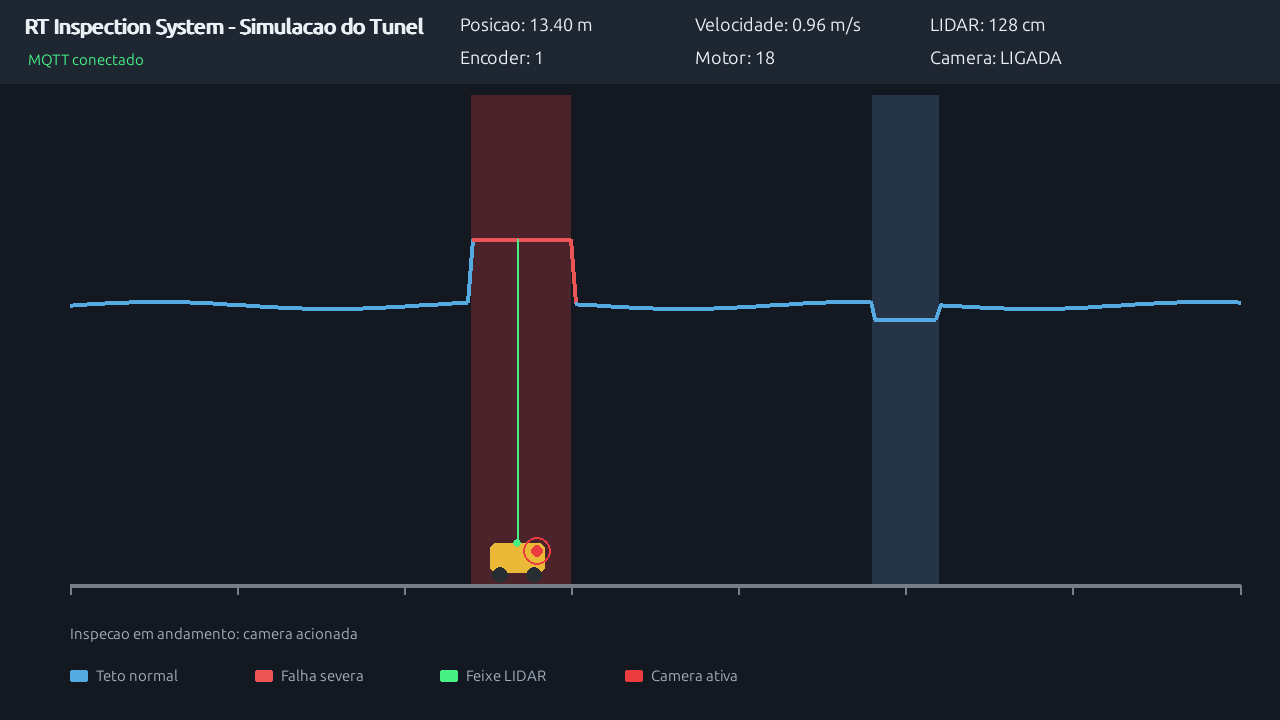
\includegraphics[width=\textwidth]{figuras/testes/simulacao_integrada.png}
    \caption{Interface de simulação na região de falha: LIDAR em 128 cm, câmera ligada e velocidade reduzida.}
    \label{fig:simulacao-final}
\end{figure}

\begin{figure}[H]
    \centering
    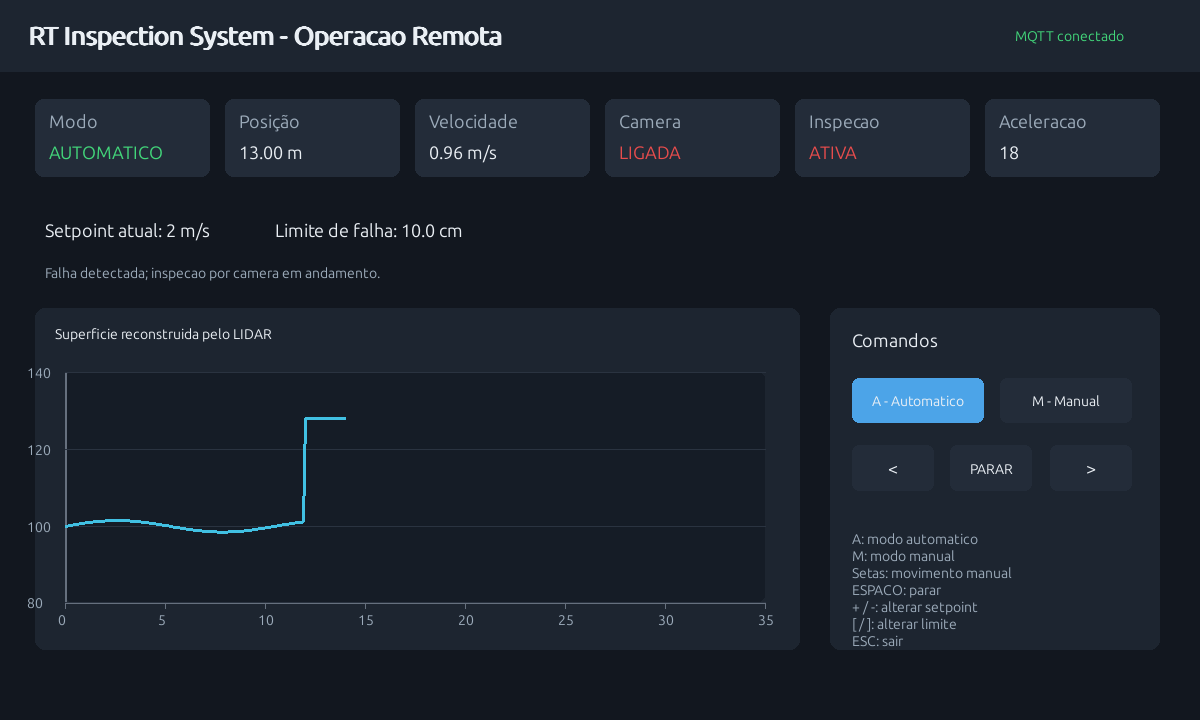
\includegraphics[width=\textwidth]{figuras/testes/operacao_remota_integrada.png}
    \caption{Operação remota exibindo inspeção ativa e descontinuidade na superfície reconstruída.}
    \label{fig:remota-final}
\end{figure}

O teste determinístico publica uma anomalia conhecida e permite verificar o evento sem depender do ruído aleatório. A Figura~\ref{fig:teste-falha} mostra a falha detectada, o início da câmera e o término do processamento. A Figura~\ref{fig:teste-csv} mostra o CSV produzido pelo pipeline.

\begin{figure}[H]
    \centering
    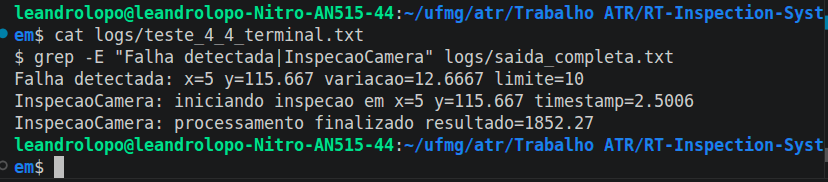
\includegraphics[width=0.92\textwidth]{figuras/testes/teste_4_4_terminal.png}
    \caption{Detecção determinística de falha e execução da tarefa de câmera.}
    \label{fig:teste-falha}
\end{figure}

\begin{figure}[H]
    \centering
    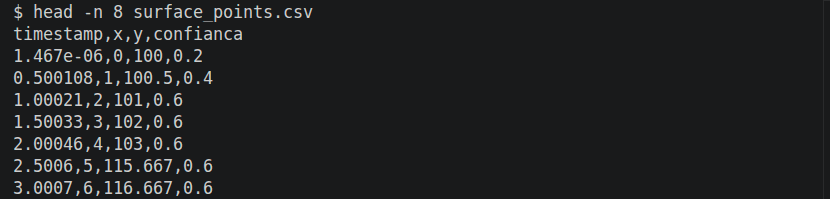
\includegraphics[width=0.92\textwidth]{figuras/testes/teste_4_3_terminal.png}
    \caption{Amostras gravadas em \texttt{surface\_points.csv}.}
    \label{fig:teste-csv}
\end{figure}

\subsection{Limites da validação}

Os testes cobrem os caminhos nominais, modos de controle, falha, finalização e parsing inválido. Não foram introduzidas perdas artificiais de pacotes, falhas de máquina ou carga competitiva extrema. Como MQTT usa QoS 0 e as filas são não limitadas, testes futuros devem incluir perda de mensagens, reconexão, saturação de filas e análise com sanitizadores de concorrência.

\section{Análise de Capacidade e Escalabilidade}

\subsection{Método de medição}

Foi criado o alvo \texttt{make benchmark}, que pré-carrega os buffers e chama as implementações reais de \texttt{DistanciaPercorrida}, \texttt{ReconstrucaoSuperficie}, \texttt{ColetorDados} e \texttt{InspecaoCamera}. Cada trecho normal processa 2.000 amostras em 20 rodadas. O tempo é medido com \texttt{steady\_clock}. Em seguida, a média, o percentil 95 e o maior resultado entre as rodadas são divididos pelo número de amostras. O benchmark também mede o custo de serialização e interpretação do JSON, mantendo os logs redirecionados para que não dominem o resultado.

Essas medidas representam custo computacional com mutexes sem contenção e dados já disponíveis. Elas não incluem atraso do broker, escalonamento entre processos, desenho da interface nem contenção do sistema operacional. Portanto, servem para dimensionamento de CPU, e não como WCET formal.

\begin{table}[H]
    \centering
    \caption{Resultados do benchmark temporal.}
    \label{tab:benchmark}
    \begin{tabular}{lrrr}
        \toprule
        \textbf{Trecho} & \textbf{Média ($\mu$s)} & \textbf{P95 ($\mu$s)} & \textbf{Máximo ($\mu$s)} \\
        \midrule
        Distância percorrida & 1,360 & 2,183 & 3,120 \\
        Reconstrução da superfície & 1,830 & 1,889 & 1,915 \\
        Coletor de dados & 12,453 & 12,688 & 12,715 \\
        JSON (serializar + interpretar) & 21,629 & 22,231 & 22,590 \\
        \midrule
        Câmera & \multicolumn{3}{c}{2.000,256 ms por evento} \\
        \bottomrule
    \end{tabular}
\end{table}

Considerando de forma conservadora a soma dos maiores valores normais da Tabela~\ref{tab:benchmark}, o processamento computacional por amostra é aproximadamente:

\[
    C_{amostra} \approx 3{,}120 + 1{,}915 + 12{,}715 + 22{,}590
    = 40{,}340\ \mu s \approx 0{,}041\ ms.
\]

Com período de 80 ms, a taxa é 12,5 amostras/s e a utilização computacional desse caminho isolado é inferior a 0,1\% de um processador lógico. Os publishers de estado e atuadores trabalham no mesmo período. Embora a câmera ocupe aproximadamente um núcleo durante 2 s, ela está separada do caminho de controle. Na máquina com 16 processadores lógicos, essa divisão manteve o controle responsivo durante a inspeção.

\subsection{Período mínimo e garantia temporal}

O menor período validado para o sistema completo é \textbf{80 ms}. Esse valor é usado pela física simulada, pelo controle, pelo comando e pelos publishers, fornecendo margem ampla sobre o custo computacional medido. Entretanto, essa validação não representa uma garantia de tempo real rígido. O protótipo executa em Linux comum com política padrão \texttt{SCHED\_OTHER}, sem prioridade de tempo real, afinidade de CPU, memória bloqueada ou medição de WCET sob todas as cargas.

O custo isolado indica que períodos computacionais menores seriam possíveis. Contudo, à medida que o período diminui, atraso do MQTT, desenho, jitter e preempções passam a ter mais influência que o próprio cálculo. Por isso, \textbf{80 ms é o menor ciclo testado e considerado seguro nesta configuração}. A adoção de um valor inferior exigiria uma campanha específica de latência e jitter. Uma garantia formal também dependeria de \texttt{SCHED\_FIFO} ou \texttt{SCHED\_RR}, prioridades por criticidade, medição de pior caso, filas limitadas e testes sob carga.

\subsection{Gargalos de escalabilidade}

\begin{itemize}
    \item \textbf{Coletor:} a confiança percorre todo o histórico. Para $N$ pontos, o custo acumulado é $O(N^2)$. Uma janela espacial ou índice por posição tornaria o custo aproximadamente constante por amostra.
    \item \textbf{Filas:} \texttt{std::queue} não possui limite nem política de descarte. Se o produtor superar o consumidor por muito tempo, memória e latência crescem. Filas circulares limitadas são mais adequadas para operação contínua.
    \item \textbf{MQTT QoS 0:} prioriza baixa sobrecarga, mas não garante entrega. QoS 1 ou numeração de sequência seria necessária se nenhuma amostra pudesse ser perdida.
    \item \textbf{Logs:} \texttt{std::cout} protegido por mutex serializa threads e pode aumentar jitter. Em produção, os logs devem ser reduzidos ou enviados a uma fila assíncrona.
    \item \textbf{Câmera:} a carga de 2 s é proposital e paralela. Em hardware com um único núcleo, ela competiria diretamente com o controle e exigiria prioridade/afinidade ou aceleração dedicada.
    \item \textbf{Broker único:} é adequado ao protótipo local. Vários robôs exigiriam prefixos por dispositivo, controle de acesso e avaliação de vazão do broker.
\end{itemize}

\section{Link para o Vídeo}

O vídeo foi produzido a partir de uma execução integrada do sistema, iniciada pelo script \texttt{run\_all.py}. A gravação reuniu a simulação do túnel e a interface de operação remota, enquanto a narração relacionou o comportamento exibido com o processamento realizado pelo núcleo C++ e com a comunicação MQTT entre os processos.

Com duração inferior a 3 minutos, o vídeo apresenta o movimento do robô em modo automático e a construção progressiva do perfil medido pelo LIDAR. Na região de falha, são mostrados o aumento da distância ao teto, a detecção da variação, o acionamento da câmera e a redução da velocidade durante a inspeção. A demonstração termina com uma alteração para o modo manual, evidenciando que os comandos enviados pela interface remota também são recebidos e aplicados pelo núcleo.

\begin{center}
    \fbox{\parbox{0.85\textwidth}{
        \centering
        \textbf{Link do vídeo no YouTube:}\\[0.3cm]
        \texttt{INSERIR AQUI O LINK DEFINITIVO DO VIDEO}
    }}
\end{center}

\clearpage
\section{Conclusão}

O projeto integrou a simulação do robô, o núcleo de processamento e a operação remota em um único fluxo de inspeção. A simulação envia encoder, LIDAR e velocidade por MQTT. A partir desses dados, o núcleo controla o movimento, calcula a posição, reconstrói o teto e aciona a câmera quando encontra uma variação acima do limite. O estado e os pontos reconstruídos retornam à interface remota e também são registrados em CSV.

Para executar esse fluxo de forma concorrente, o núcleo foi dividido em 11 threads com responsabilidades definidas. Os mutexes protegem os estados compartilhados, enquanto as filas e variáveis de condição coordenam produtores e consumidores sem espera ocupada. As tarefas de controle seguem um período de 80 ms, e o processamento de câmera permanece em uma thread separada para não bloquear diretamente a malha de navegação. Essa organização permitiu relacionar a implementação aos conceitos de concorrência, sincronização, temporização e IPC estudados na disciplina.

Os testes exercitaram o percurso nominal, os modos automático e manual, a reconstrução, a detecção de falha, a câmera e o encerramento das threads. Nas configurações avaliadas, o custo computacional do pipeline normal permaneceu muito abaixo do período adotado, tornando 80 ms o menor ciclo validado para o sistema completo. O resultado confirma o funcionamento do protótipo, mas não caracteriza uma garantia de tempo real rígido. Para aproximar a solução de uma aplicação crítica, ainda seria necessário limitar as filas, melhorar a complexidade do coletor, tratar perdas e reconexões MQTT e executar as tarefas com políticas e prioridades de tempo real.

\clearpage
\appendix
\section{Código-fonte}

Este apêndice incorpora os arquivos utilizados no projeto. Os códigos são lidos diretamente do repositório durante a compilação deste relatório.

\subsection{Compilação}
\lstinputlisting[style=textstyle]{Makefile}

\subsection{Inicialização dos processos}
\lstinputlisting[style=pythonstyle]{run_all.py}

\section{Cabeçalhos C++}
\codigo{buffers.hpp}{include/buffers.hpp}
\codigo{log.hpp}{include/log.hpp}
\codigo{mqtt\_topics.hpp}{include/mqtt_topics.hpp}
\codigo{shared\_state.hpp}{include/shared_state.hpp}
\codigo{tasks.hpp}{include/tasks.hpp}
\codigo{time\_utils.hpp}{include/time_utils.hpp}
\codigo{types.hpp}{include/types.hpp}

\section{Núcleo C++}
\codigo{main.cpp}{src/main.cpp}
\codigo{comando\_navegacao.cpp}{src/comando_navegacao.cpp}
\codigo{controle\_navegacao.cpp}{src/controle_navegacao.cpp}
\codigo{distancia\_percorrida.cpp}{src/distancia_percorrida.cpp}
\codigo{reconstrucao\_superficie.cpp}{src/reconstrucao_superficie.cpp}
\codigo{coletor\_dados.cpp}{src/coletor_dados.cpp}
\codigo{inspecao\_camera.cpp}{src/inspecao_camera.cpp}
\codigo{mqtt\_sensor\_subscriber.cpp}{src/mqtt_sensor_subscriber.cpp}
\codigo{mqtt\_command\_subscriber.cpp}{src/mqtt_command_subscriber.cpp}
\codigo{mqtt\_actuator\_publisher.cpp}{src/mqtt_actuator_publisher.cpp}
\codigo{mqtt\_state\_publisher.cpp}{src/mqtt_state_publisher.cpp}
\codigo{mqtt\_surface\_publisher.cpp}{src/mqtt_surface_publisher.cpp}
\codigo{simulacao\_sensores.cpp}{src/simulacao_sensores.cpp}
\codigo{log.cpp}{src/log.cpp}
\codigo{time\_utils.cpp}{src/time_utils.cpp}

\section{Simulação e Operação Remota}
\codigopython{simulation\_gui.py}{simulation/simulation_gui.py}
\codigopython{simulation\_physics.py}{simulation/simulation_physics.py}
\codigopython{simulation\_test.py}{simulation/simulation_test.py}
\codigopython{actuator\_receiver\_test.py}{simulation/actuator_receiver_test.py}
\codigopython{remote\_gui.py}{remote_operation/remote_gui.py}

\section{Benchmark Temporal}
\codigo{benchmark\_temporal.cpp}{tests/benchmark_temporal.cpp}

\end{document}
